\documentclass[tikz,border=10pt,12pt]{standalone}
% Shared preamble for standalone-compiled dc_paper figures.
% Copies just the bits of dc_paper.tex's preamble that figures need.

\usepackage{amsmath,amssymb,amsthm,mathtools,bm}
\usepackage{siunitx}
\sisetup{detect-all,group-separator={,},per-mode=symbol}

\usepackage[T1]{fontenc}
\usepackage{xcolor}
\usepackage{enumitem}
\usepackage{mathpazo}                % Palatino body + matching math
\usepackage[scaled=0.92]{helvet}     % Helvetica sans
\usepackage{courier}                 % monospace
\usepackage{microtype}

% --- IA brand colour palette (must match dc_paper.tex) ---
\definecolor{iadark}{HTML}{1B1815}
\definecolor{iabone}{HTML}{FAFAF7}
\definecolor{iaaccent}{HTML}{A04A1F}
\definecolor{iataupe}{HTML}{F2EDE6}
\definecolor{iarule}{HTML}{3A332D}
\definecolor{iagrey}{HTML}{5A524A}

% --- graphics ---
\usepackage{tikz}
\usepackage{circuitikz}
\usepackage{pgfplots}
\pgfplotsset{compat=1.18}
\usetikzlibrary{arrows.meta,positioning,shapes.geometric,calc,fit,
                decorations.pathreplacing,decorations.markings,
                shadows.blur,backgrounds}

% --- math macros from dc_paper.tex preamble (figures use them) ---
\newcommand{\E}{\mathbb{E}}
\newcommand{\Var}{\operatorname{Var}}
\newcommand{\Cov}{\operatorname{Cov}}
\newcommand{\Cor}{\operatorname{Cor}}
\newcommand{\Prb}{\mathbb{P}}
\newcommand{\R}{\mathbb{R}}
\newcommand{\N}{\mathbb{N}}
\newcommand{\1}{\mathbf{1}}
\newcommand{\VaR}{\operatorname{VaR}}
\newcommand{\TVaR}{\operatorname{TVaR}}
\newcommand{\ES}{\operatorname{ES}}
\newcommand{\dd}{\mathrm{d}}
\newcommand{\given}{\,\vert\,}
\newcommand{\set}[1]{\left\{#1\right\}}
\newcommand{\norm}[1]{\left\Vert #1 \right\Vert}
\DeclareMathOperator*{\argmin}{arg\,min}
\DeclareMathOperator*{\argmax}{arg\,max}

% \textwidth has no meaning in standalone class; give it a value matching
% the paper's A4 + 1-inch margins so any leftover \resizebox{\textwidth}
% gracefully sizes the figure to that nominal width.
\setlength{\textwidth}{15.92cm}

\begin{document}
\pagecolor{iabone}
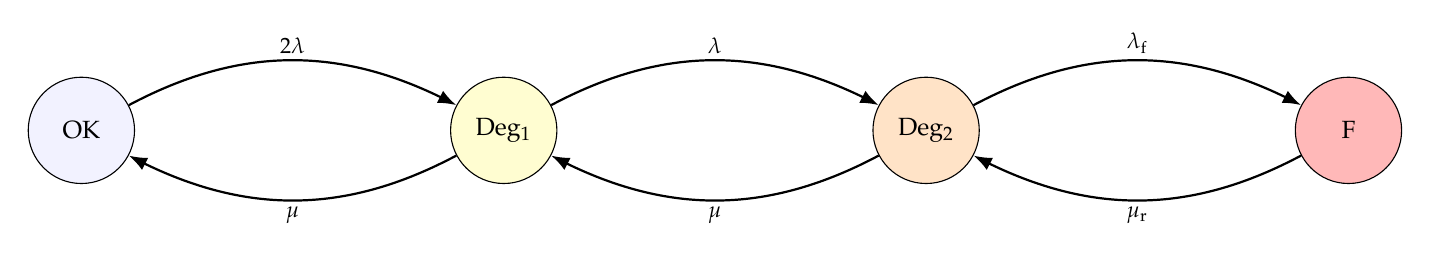
\begin{tikzpicture}[
  >=Latex,
  node distance=3.6cm and 4.0cm,
  state/.style={draw,circle,minimum size=1.35cm,inner sep=1pt,
                font=\small,fill=blue!5},
  every edge/.style={draw,thick,->,>=Latex},
  every node/.style={font=\footnotesize},
  ratelbl/.style={midway,font=\footnotesize,inner sep=2pt,fill=white,
                  fill opacity=0.85,text opacity=1}
]
\node[state]                                  (S0) {OK};
\node[state,right=of S0,fill=yellow!18]       (S1) {Deg$_1$};
\node[state,right=of S1,fill=orange!22]       (S2) {Deg$_2$};
\node[state,right=of S2,fill=red!28]          (SF) {F};

% Forward arrows bend upward (label above the upper arc); reverse arrows
% bend left=28 in the leftward direction, which curves them downward, so
% their label goes below the lower arc. Semi-opaque white background on
% the labels keeps them legible even where they get close to an arc.
\draw (S0) edge[bend left=28]  node[ratelbl,above] {$2\lambda$}                 (S1);
\draw (S1) edge[bend left=28]  node[ratelbl,below] {$\mu$}                      (S0);
\draw (S1) edge[bend left=28]  node[ratelbl,above] {$\lambda$}                  (S2);
\draw (S2) edge[bend left=28]  node[ratelbl,below] {$\mu$}                      (S1);
\draw (S2) edge[bend left=28]  node[ratelbl,above] {$\lambda_{\mathrm{f}}$}     (SF);
\draw (SF) edge[bend left=28]  node[ratelbl,below] {$\mu_{\mathrm{r}}$}         (S2);
\end{tikzpicture}%
\end{document}
